
%(BEGIN_QUESTION)
% Copyright 2011, Tony R. Kuphaldt, released under the Creative Commons Attribution License (v 1.0)
% This means you may do almost anything with this work of mine, so long as you give me proper credit

Identify which mathematical formula best describes the function of this pneumatic relay mechanism, assuming the positions of all bellows are drawn to scale:

$$\includegraphics[width=15.5cm]{i00939x01.eps}$$

$$z = {x + y \over 2} - 3k$$

$$z = {x - y \over 3} + 2k$$

$$z = 2y + x + {k \over 3}$$

$$z = {y \over 3} + {2x \over 3} - k$$

$$z = 2{k + x} - 3y$$

$$z = 2(y - x) - 3k$$

Also, identify whether this mechanism is {\it force balance} or {\it motion balance}.

\vfil 

\underbar{file i00939}
\eject
%(END_QUESTION)





%(BEGIN_ANSWER)

This is a graded question -- no answers or hints given!

%(END_ANSWER)





%(BEGIN_NOTES)

The very first analytical step you should do when examining a pneumatic mechanism is to figure out whether it is a {\it force-balance} or a {\it motion-balance}, because this profoundly impacts how we must view the inputs and outputs.  The best test for this is to apply our ``simplifying assumption'' of the baffle/nozzle gap remaining absolutely constant and then determine whether or not the mechanism is able to move.  Since the bottom end of the flapper beam is anchored at a pivot, and the top end is the constant gap (in relation to a nozzle that is also anchored and therefore stationary), we can see that the beam cannot move so long as that gap is constant.  No motion possible means {\bf force-balance} for this mechanism.

\vskip 10pt

Now that we know it is a force-balance mechanism, we know we must view all the inputs in terms of {\it how hard they push}, not {\it how far they move}.  The output bellows clearly has a lot of leverage, being located far from the bottom of the flapper beam (long lever length = minimal force needed).  The tension spring's force $k$ is applied to the beam over the same leverage, which means that force will have considerable effect over the output pressure.  We may also conclude that the spring tension $k$ must be a negative quantity in this mechanism's mathematical function since it works in the same direction as the output bellows and therefore allows the output bellows to achieve force-balance with {\it less} air pressure.  

Given the fact that the output bellows enjoys more leverage than either bellows $x$ or $y$, we may conclude that the air pressure inside the output bellows will be less than that of either $x$ or $y$ in a balanced state.  In other words, only a {\it fraction} of the pressure applied to $x$ or $y$ will manifest on the output of this mechanism.  Following this logic, we may discard any formula where the output ($z$) is some multiple of one or both of the inputs ($x$ and/or $y$) -- instead, $z$ must be a function of some {\it fraction} of both $x$ and $y$. 

\vskip 10pt

We can also see that input $x$ has more of an advantage than input $y$, its bellows being located farther from the pivot (and therefore having more force-leverage).  Thus, the effect of input pressure $x$ will be greater on output $z$ than input pressure $y$.  Following this logic, we need to look for a formula where $x$'s coefficient is larger than $y$'s coefficient.

\vskip 10pt

Finally, we can see that both the $x$ bellows and the $y$ bellows push on the flapper beam in the same direction, which tells us both of these variables must have the same {\it sign} in the formula.  Therefore, we can eliminate any formula that has $x-y$, $y-x$, or anything else like that.

\vskip 10pt

Putting all these criteria together, we see only one possible formula in the list which could describe this mechanism's behavior:

$$z = {y \over 3} + {2x \over 3} - k$$

%INDEX% Relay, computational: matching mathematical function to pneumatic mechanism

%(END_NOTES)


